% \textbf{Title: Fields 14}

A moving electron with charge -e travels along the path shown, and passes through a region of electric field. There are no other charges present. The electric field is zero everywhere except in the gray region.

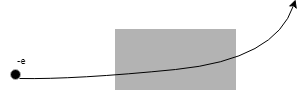
\includegraphics[width=2.5in]{../../Images/FieldsEBHQ14.png}

What is a possible direction of the electric field in the region where the field is non-zero?\\

a. Out of the plane, $\odot$.

b. Into to the plane, $\otimes$.

c. Upwards, $\uparrow$.

*d. Downwards, $\downarrow$.

e. I do not know.\\
